\section{Evaluation}
\label{sec:eval}
% a simple tool for multiple choice dataset evaluation and correction
We first show the experimental setup and then give the results on
i) extraneous feature classification,
ii) cue discovery on 3 datasets,
iii) feature sensitivity of 3 models as well as their PLMs on the 3 datasets.
Finally, we provide some case study. 
%The whole framework has been implemented into an online demo at
%\url{http://anonymized.for.blind.review}.
All models are implemented and tested on an RTX 2080Ti GPU with 11G RAM.

\begin{table*}[!th]
\scriptsize
\centering
\begin{tabular}{lcccccccc}\hline
Dataset & Type & Data Size & Train/Test & Human Acc & BT Acc & RB Acc & XL Acc & AB Acc \\ 
 	&	&	& Ratio	& (\%) \\ \hline
SNLI     &CLS   &  570K     & 56:1               &80.0\\
QNLI     &CLS    & 11k         &  19:1           &80.0\\
MNLI     &CLS     & 413k       &  40:1             &80.0\\
ROCStory & MCQ & 3.9k         & 1:1            &100.0  \\
COPA     &MCQ    & 1k           &  1:1         & 100.0     \\
SWAG     &MCQ   & 113k       &  4:1             & 88.0\\
RACE     & MCQ   & 100k      &  18:1              &94.5\\
RECLOR   &MCQ    &  6k          &  9:1           &63.0\\
%CQA      &MCQ   & 12k        &  9:1                &88.9\\
ARCT     &MCQ    & 2k         & 3:1                &79.8\\
ARCT\_adv& MCQ & 4k         & 3:1                 & -\\
\hline
\end{tabular}
\caption{10 Datasets. Data size refers to the number of questions
in each dataset. CLS=Classification. MCQ=Multiple Choice Questions. 
By our definition, $k$-way MCQs will be split into $k$ instances 
in preprocessing.}\label{tab:datasets} 
\end{table*}

\KZ{Add some new datasets including aNLI.} 
These datasets can mainly be classified into two types of tasks. 
SNLI, QNLI, and MNLI are classification tasks, while 
ROCStory, COPA~\cite{roemmele2011choice}, SWAG~\cite{zellers2018swag}, 
RACE~\cite{lai2017race}, 
RECLOR~\cite{yu2020reclor}, %CQA~\cite{talmor2019commonsenseqa}, 
ARCT and ARCT\_adv~\cite{schuster2019towards} are
multiple choice reasoning tasks. 
We set the minimum number appearance of a feature
in either the training or the test set to be 5 to qualify as a cue.

\subsection{Setup} 
We evaluate this framework on 10 popular NLR datasets and
4 well-known PLM models, namely BERT (BT), RoBERTA (RB), XLNet (XL) and Albert (AB)
on these datasets. All these datasets except for SWAG and RECLOR are collected
through crowdsourcing. SWAG is generated from an LSTM-based language model.
Specifications of the datasets are listed in \tabref{tab:datasets}.


%Because CQA has very short hypotheses, only word cues apply.

%In~\secref{sec:extract}, we choose to use CP as feature metric because from~\figref{fig:d_figure} we find that 
%Pearson Correlation Coefficient(PCC) of accuracy deviation score ($\mathcal{D}$)
%\begin{equation}
%    \mathcal{D} = {Acc} - {Majority}\footnote{Majority is the accuracy with majority voting.}
%\end{equation}
%between a logistic regression trained with CP and hypothesis-only models (BERT and fastTest) 
%is up to 97.17\% for fastText and 97.34\% for BERT which indicates CP is a good feature evaluation score 
%for a dataset. 
%
% In addition, we choose to assign $k$ to 10 which means for Word feature, we only consider 
%top 10 works with high feature score. 
%The threshold $\sigma$ for decide whether a feature dataset is 
%big enough is 5. 
%
%\subsection{Baselines}
%
%\paragraph{Frequency(Freq)}
%The most simple but straight measurement is the number of co-occurrences
%of the words and labels in the data.
%\begin{equation}
%    f_{Freq}^{(w,l)} = \#(w, l)
%\end{equation}
%
%\paragraph{Point-wise Mutual Information (PMI)}
%
%PMI is a widely used method for association measurement in information theory and statistics.
%We estimate the probability:
%\begin{equation}
%p(l) = \frac{\#(l)}{\#(\mathcal{L})}, p(l|w) = \frac{\#(w, l)}{\#(w)},
%\end{equation}
%where $\#(\mathcal{L}) = \sum_{l\in \mathcal{L}} \#(l)$.
%The PMI score of token $w$ with respect to label $l$ is
%\begin{equation}
%    f_{PMI}^{(w,l)} = \log \frac{p(l|w)}{p(l)}
%\end{equation}
%
%\paragraph{Local Mutual Information (LMI)}
%
%Considering the frequency of tokens can influence models with different weight and inspired
%by \citeauthor{schuster2019towards}'s work,
%we estimate the probability by
%\begin{equation}
%    p(w, l) = \#(w, l) / \sum_{i=1}^{|\mathcal{N}|}\#(w_i).
%\end{equation}
%The LMI of token $w_k$ with respect to label $l$ is
%\begin{equation}
%    f_{LMI}^{(w,l)} = p(w, l)\log \frac{p(l|w)}{p(l)}.
%\end{equation}
%
%\paragraph{Ratio Difference (RF)}
%\begin{equation}
%    f_{RF}^{(w,l)} = \left|\frac{\#(w, l)}{\#(w, \mathcal{L'})} -
%    \frac{\#(l)}{\#(\mathcal{L'})}\right|
%\end{equation}
%
%\paragraph{Angle Difference (AD)}
%Angle Difference is similar to \textit{Ratio Difference} except that we take arc-tangent function.
%\begin{equation}
%    f_{AD}^{w,l} = \left| \arctan\frac{\#(w, l)}{\#(w, \mathcal{L'})} -
%    \arctan \frac{\#(l)}{\#(\mathcal{L'})} \right|
%\end{equation}
%
%\paragraph{Cosine(Cos)}
%%We imply calculation of the cosine distance between the two vectors.
%Let $v_w=[\#(w, l), \#(w, \mathcal{L'})]$ and $v_l = [(\#(l), \#(\mathcal{L'})]$,
%two vectors on a 2D plane.
%Intuitively, if $v_w$ and $v_l$ are co-linear, $w$ leaks no spurious information.
%Otherwise, $w$ is suspected to be a spurious cue as it tends to appear
%more with a specific label $l$.
%\begin{equation}
%    f_{Cos}^{(w,l)} = \cos(v_w, v_l)
%\end{equation}
%
%\paragraph{Weighted Power(WP)}
%\begin{equation}
%    f_{WP}^{(w,l)} = (1-f_{Cos}^{l})\#(w)^{f_{Cos}^{l}}
%\end{equation}
%
%We further define accuracy deviation score ($\mathcal{D}$)
%\begin{equation}
%    \mathcal{D} = {Acc} - {Majority},
%\end{equation}
%where $Acc$ is the prediction accuracy of a simple logistic regression
%model trained on the CP feature of all words or of a hypothesis-only
%model, and $Majority$ is the accuracy of vote by majority.
%As \figref{fig:d_figure} shows, accuracy of the linear model using 
%the CP features is very similar to the more complex hypothesis-only models 
%(Pearson score of 97.17\% for fastText and 97.34\% for Bert), 
%which indicates CP is a good choice of word feature.
%
%\begin{figure}[th]
%\centering
%\includegraphics[width=0.9\columnwidth]{picture/d_figure.pdf}
%\caption{Deviation scores for three prediction models on all 12 datasets. 
%``Our'' means our logistic regression model. \KZ{Change this to a 
%distogram}}
%\label{fig:d_figure}
%\end{figure}
%

%\subsection{Hypothesis-only Tests}
%As a comparison to our framework, we first show the hypothesis-only test results
%on our 4 models and 10 datasets. In this test, we apply the models trained on
%full training data (with both premise and hypothesis) of the 10 datasets, and
%test their accuracies on the hypothesis-only test data (by stripping
%the premises from the questions in the test set). \tabref{tab:hypoonly}
%shows the results, compared with the original accuracies using the full
%test data. 
%
%\begin{table}[th]
%\centering
%\scriptsize
%\begin{tabular}{c|c|c|c|c|c} \hline
%Dataset & Majority & FT & ES & BT & RB \\ \hline
%\multirow{2}{*}{SNLI} & \multirow{2}{*}{33.3} &  54.43& 87.44  &  90.56 & 91.86 \\
%	& &   59.83  &    59.55  &  45.7& 45.29 \\ \hline
%\multirow{2}{*}{QNLI}  & \multirow{2}{*}{50} &  67.17 & 61.60  &  86.42 & 90.37 \\
%	&  &66.4   &  57.45    & 55.16 & 52.91 \\ \hline
%\multirow{2}{*}{MNLI} & \multirow{2}{*}{33.3} & 47.2  & 54.63  & 83.42  & 87.21 \\
%	& & 52.46&   54.57  &   36.66   &  37.84  \\ \hline
%\multirow{2}{*}{ROCStory} & \multirow{2}{*}{50} & 61.73  &  62.91 &  86.85 &  91.55\\
%	& &   60.24  &   59.88  & 56.44 & 74  \\ \hline
%\multirow{2}{*}{COPA}   & \multirow{2}{*}{50} & 48  & 53.8  &  67.4 & 69 \\
%	& &   48.4    &  51.4& 60 & 58.4\\ \hline
%\multirow{2}{*}{SWAG}  & \multirow{2}{*}{25} & 27.79  &  68.95 &  77.58 &  81.89\\
%	& &  27.82  &   50.62   &  53.66& 58.42 \\ \hline
%\multirow{2}{*}{RACE}  & \multirow{2}{*}{25} & 29.87  &  31.35 & 29  & 29.69 \\
%	& &    31.27  &  29.83    & 30.09 &  24.48\\ \hline
%\multirow{2}{*}{RECLOR} & \multirow{2}{*}{25} & 32.2  & 30.96  &  45 & 54.2 \\
%	& &   31.6 &  30.2    &40.2 & 32.2 \\ \hline
%\multirow{2}{*}{ARCT}& \multirow{2}{*}{50} &  50.23 & 47.52  & 65.76  & 77.25 \\ 
%	& &  50.23   &  49.77    & 62.83 & 65\\ \hline
%\multirow{2}{*}{ARCT\_adv}& \multirow{2}{*}{50} & 50  &50 & 50.33  & 50 \\
%	&  &  50  &  50    & 50 & 50\\ \hline
%\end{tabular}
%\caption{Hypothesis-only Tests (\%). The number on the above in each cell is the original accuracy on
%full test data; on the bottom is the accuracy on hypothesis-only tests.}\label{tab:hypoonly}
%\end{table}
%
%We further plot the four models hypothesis-only accuracies against voting by majority
%results in \tabref{tab:hypoonly} in \figref{fig:ending1}. 
%This figure depicts the ``weakness'' of the datasets to these models. 
%The higher the bars, the weaker the dataset. We can see that SWAG, SNLI and MNLI
%are generally easier, whereas ARCT\_ADV is a hard task (the deviation results
%approach to zero).
%
%Next, we plot the differences between the model accuracies on the full test data
%and the accuracies on the hypothesis-only data in \figref{fig:ending2}. 
%This experiment evaluates the robustness of the models. 
%We see that the bars for FastText or ESIM are very short, while
%the bars are much longer for BERT and RoBERTA. This shows that from 
%the hypothesis-test point of view, BERT and RoBERTA are more robust 
%against the artifacts in the datasets, because the duo do not 
%perform as well when given only
%the ending of the questions. 
%These preliminary results serve as the basis for our findings next.
%
%\begin{figure}[th]
%\centering
%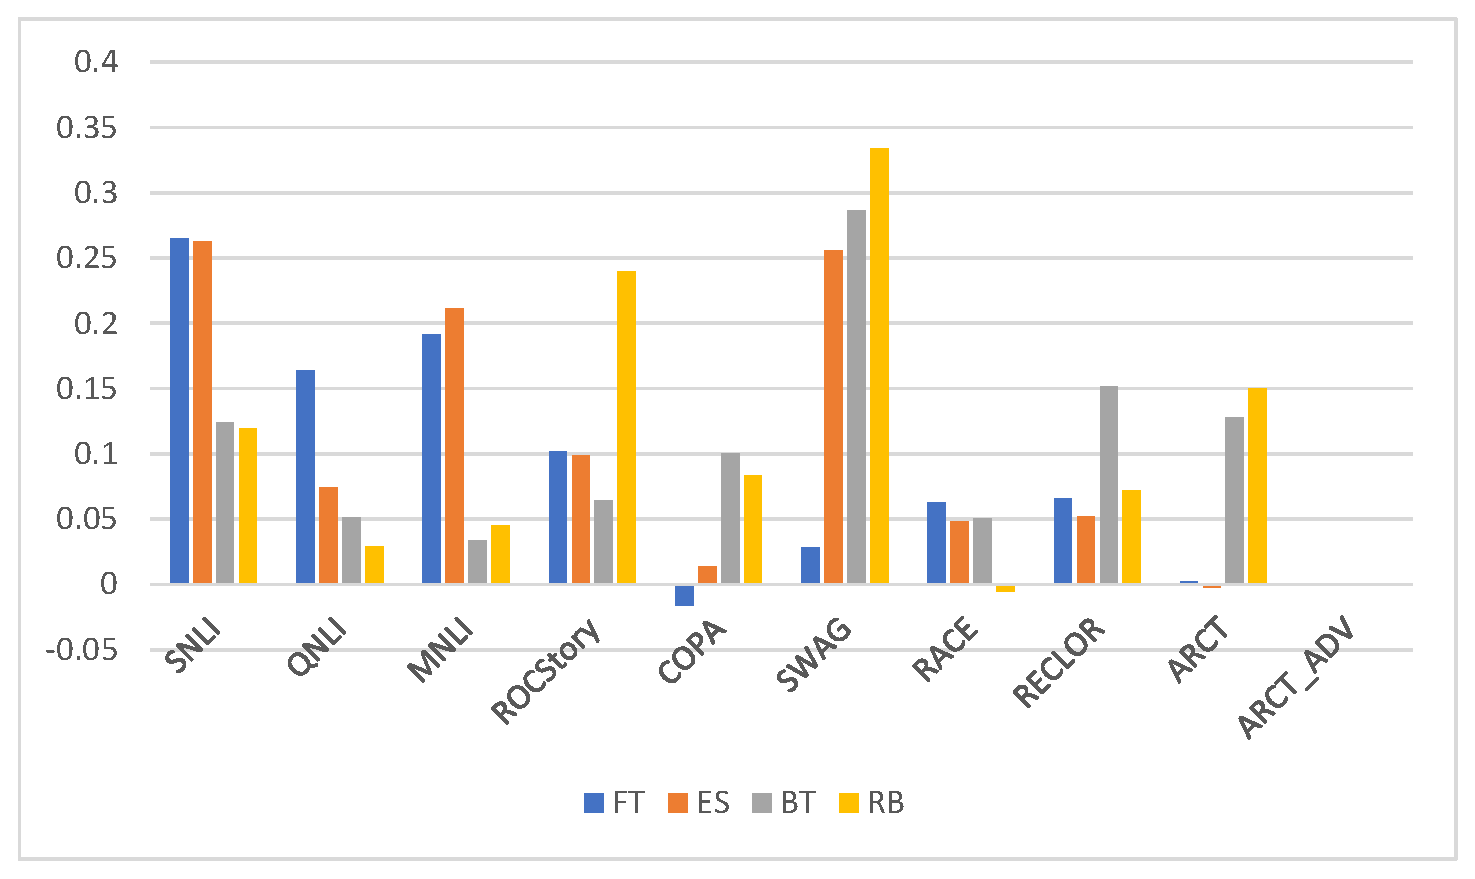
\includegraphics[width=\columnwidth]{picture/ending1.eps}
%\caption{Four models' hypothesis-only tests accuracies beyond vote by majority (hypo-only
%acc $-$ majority acc)}
%\label{fig:ending1}
%\end{figure}
%
%\begin{figure}[th]
%\centering
%\includegraphics[width=\columnwidth]{picture/ending2.eps}
%\caption{Four models' full test accuracies above hypothesis-only tests accuracies (full acc $-$
%hypo-only acc)}
%\label{fig:ending2}
%\end{figure}
%
\subsection{Extraneous Feature Classification}

\begin{table}[ht!]
\centering
\begin{tabular}{|c|r|r|r|r|} 
\hline 
Feature & RocStory & COPA & ARCT & RECLOR \\ \hline \hline
Word &	& 	&	&  \\ \hline
Sent.&	& 	&	&  \\ \hline
Tense &	& 	&	&  \\ \hline
Neg. &	& 	&	&  \\ \hline
Over.&	& 	&	&  \\ \hline
NER&	& 	&	&  \\ \hline
Typos &	& 	&	&  \\ \hline
All &	& 	&	&  \\ \hline
\end{tabular}
\caption{Classification accuracies by the features and overall: In each cell,
first number refers to classifier by semantic similarity; second number
refers to classifier by NLI.}
\label{tab:extra}
\end{table}

\KZ{What is the train/test split? How did you label it?}
Because classifier X has an overall better accuracy than Y, we will use X in the 
remaining experiments in this section.

\subsection{Cues in Datasets}

We first filter the training and test data for each dataset leaving features with
at least a support of X. Then we rank these features, all 248 of them using Algorithm X.
\tabref{tab:bias} shows the top 20 cues we discovered along with their cue scores
for each of the 10 datasets. ARCT\_adv is an adversarial dataset
and is known to be well balanced on purpose. As a result, we only managed to find one cue
which is OVERLAP and its cueness score is very low. This is not surprising, because
OVERLAP is the only ``second-order'' feature in our list of linguistic features that
is concerned with tokens in both the premise and hypothesis, and likely escaped from
the data manipulation by the creator. 

\begin{table}[th]
\centering
\scriptsize
\begin{tabular}{|cc|cc|cc|cc|} \hline
\multicolumn{2}{|c|}{ROC} & \multicolumn{2}{c|}{COPA}& \multicolumn{2}{c|}{ARCT} & \multicolumn{2}{c|}{RECLOR} \\ \hline 
 ``sleeping'' & 13.95 & ``sleeping'' & 30.3 & ``sleeping'' & 6.81 & ``sleeping'' & 4.87 \\\hline           
 ``no'' & 13.33 & ``no'' & 18.09 &``no'' &3.32 & ``no'' & 2.05 \\
\hline 
\end{tabular}
\caption{Top cues and their cueness score for 4 datasets.}\label{tab:bias}
\end{table}

In most of the datasets, the top 5 cues discovered are word features,
but besides OVERLAP, we do see NEGATION and TYPO showing up
in the lists. In fact, SENTIMENT and NER features would have shown up
if we expanded the list to top 10. It is also interesting to see several features previously
reported to be biased by other works, such as ``not'' and NEGATION in
ARCT, ``no'' in MNLI and SNLI, and ``like'' in ROCStory.  Especially in
MNLI, all the five cues discovered are related to negatively toned words,
suggesting significant human artifacts in this datasets.
 
In the results, we also identify that some of the word cues are indicative of
certain syntactic/semantic/sentiment patterns in the questions. For example, ``because'' in SNLI
indicates a causal-effect structure; ``like'' in ROCStory indicates positive sentiment;
``probably'' and ``may'' in RACE indicate uncertainty, etc. 

If we sum up the top 5 cueness scores for each dataset, we find that
overall SNLI, RACE, ROCStory and MNLI carry more cueness than others,
while ARCT\_adv has the smallest cueness. 
%This result is generally consistent with our findings in the hypothesis-only test (see \figref{fig:ending1})
%earlier,
%though now we can pinpoint what causes the weaknesses in these four
%datasets.  The only exception is SWAG, which didn't emerge as a very
%weak dataset in the experiment here, but was found very biased in
%the hypothesis-only test. The reason is SWAG is the biggest dataset
%among the ten and we discovered more cues in it than
%the other 9 combined. Therefore, the top 5 cues are insufficient
%to represent the full scale of its weakness, which is showed by
%the hypothesis test as it gives the full picture.

%\begin{figure*}[th]
%\centering
%\begin{subfigure}[b]{0.3\textwidth}
%\centering
%\includegraphics[width=\columnwidth]{picture/no_mnli.eps}
%\caption{Cue ``no'' in MNLI}
%\label{fig:cue_no}
%\end{subfigure}
%\hfill
%\begin{subfigure}[b]{0.3\textwidth}
%\centering
%\includegraphics[width=\columnwidth]{picture/above_arct.eps}
%\caption{Cue ``above'' in ARCT}
%\label{fig:cue_above}
%\end{subfigure}
%\hfill
%\begin{subfigure}[b]{0.3\textwidth}
%\centering
%\includegraphics[width=\columnwidth]{picture/threw_roc.eps}
%\caption{Cue ``threw'' in ROCStory}
%\label{fig:cue_threw}
%\end{subfigure}
%\caption{Three test examples for distribution comparison with 4 different models}
%\label{fig:cue_result}
%\end{figure*}
%\begin{figure}[th]
%\centering
%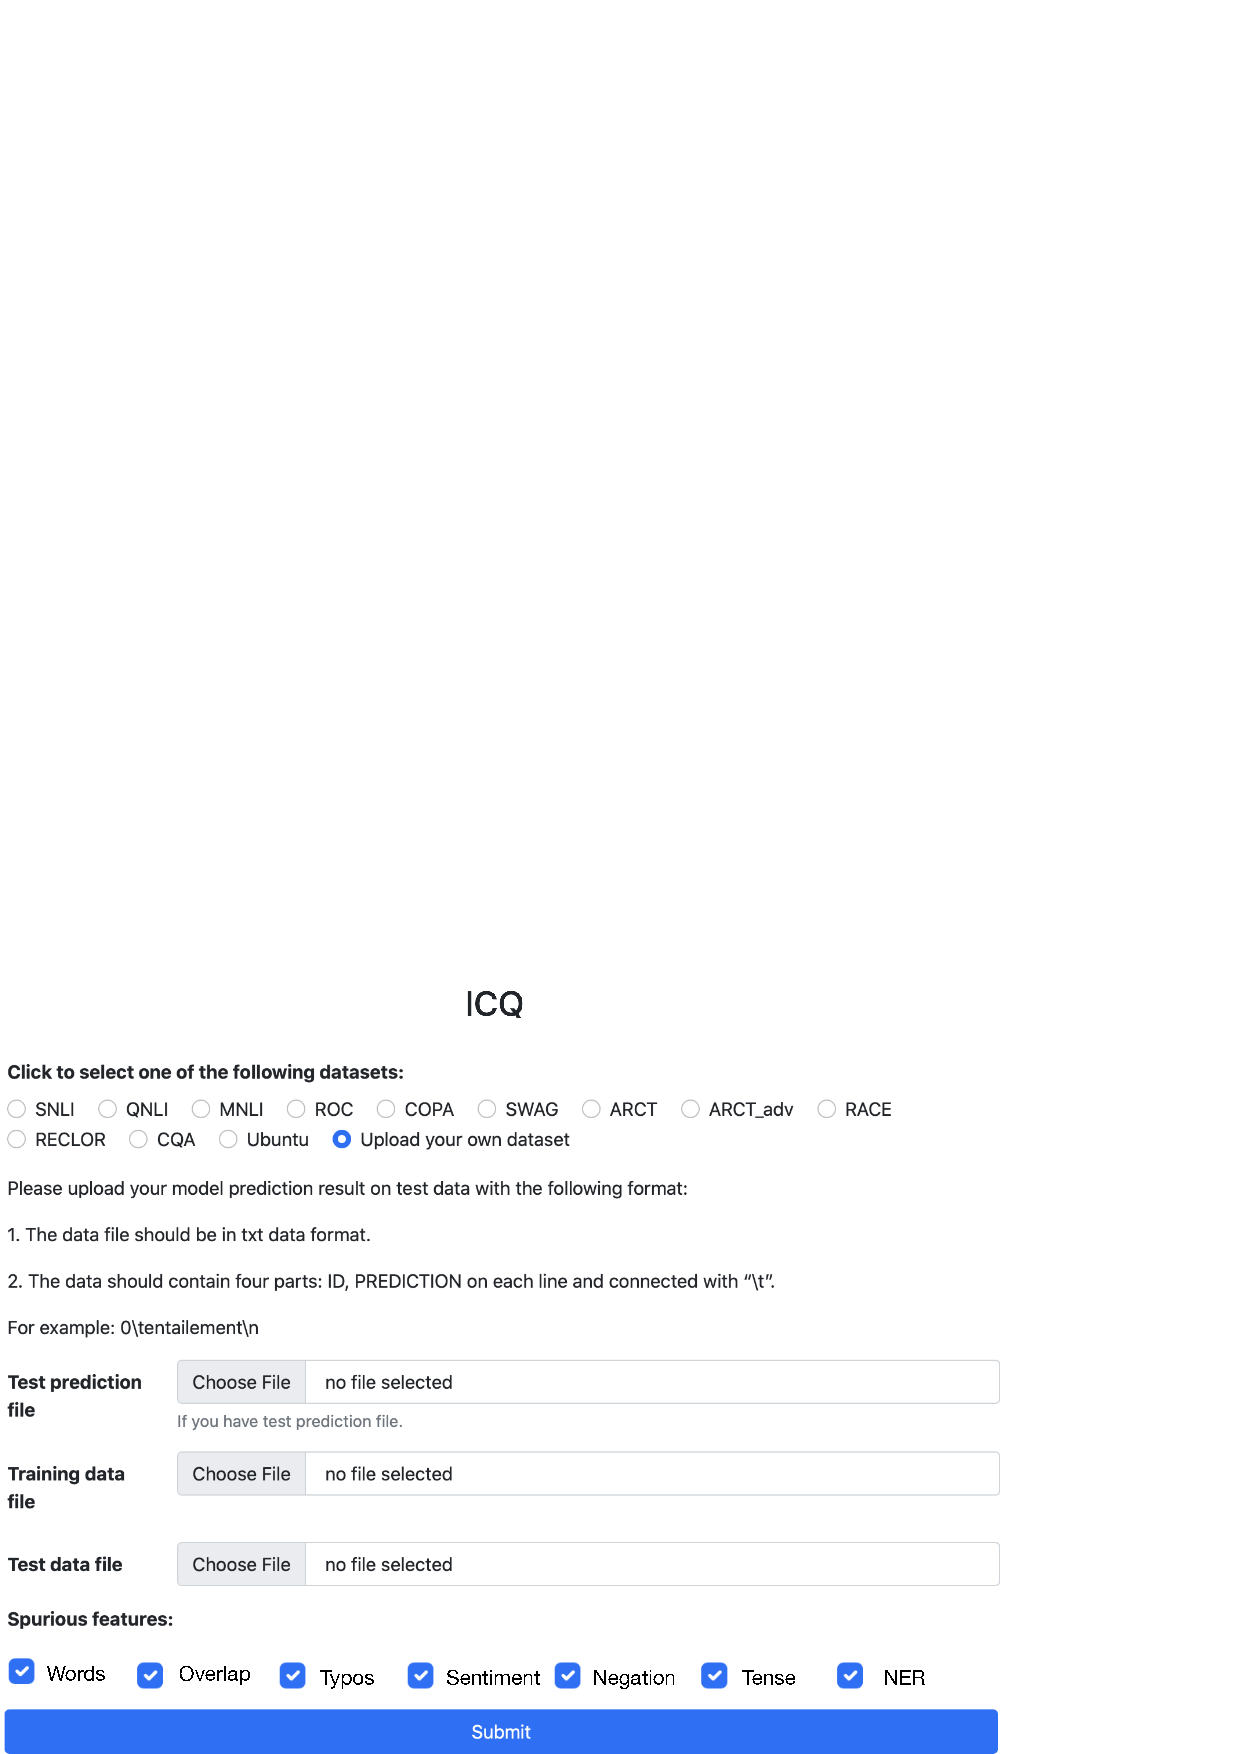
\includegraphics[width=1.0\columnwidth]{picture/dataset.jpg}
%\caption{Dataset Evaluation Panel}
%\label{fig:dataset}
%\end{figure}

\subsection{Sensitivity to Extraneous Features in Models}

We show the top sensitive features in four tables, each for a dataset.

\begin{table*}[th]
\centering
\scriptsize
\begin{tabular}{|cc|cc|cc|cc|cc|cc|cc|cc|} \hline
\multicolumn{2}{|c|}{BT} & \multicolumn{2}{c|}{BT$_0$} &\multicolumn{2}{c|}{RB}& \multicolumn{2}{c|}{RB$_0$}
	&\multicolumn{2}{c|}{XL} & \multicolumn{2}{c|}{XL$_0$} & \multicolumn{2}{c|}{AB} & \multicolumn{2}{c|}{AB$_0$} \\ \hline \hline
 ``sleeping'' & 13.95 & ``sleeping'' & 30.3 & ``sleeping'' & 6.81 & ``sleeping'' & 4.87 &``sleeping'' & 13.95 & ``sleeping'' & 30.3 & ``sleeping'' & 6.81 & ``sleeping'' & 4.87  \\\hline           
 ``no'' & 13.33 & ``no'' & 18.09 &``no'' &3.32 & ``no'' & 2.05 & ``no'' & 13.33 & ``no'' & 18.09 &``no'' &3.32 & ``no'' & 2.05 \\
\hline 
\end{tabular}
\caption{4 models + their pretrained version (denoted as $M_0$) 
and their most sensitive extraneous features on ROC.}\label{tab:roc}
\end{table*}

\begin{table*}[th]
\centering
\scriptsize
\begin{tabular}{|cc|cc|cc|cc|cc|cc|cc|cc|} \hline
\multicolumn{2}{|c|}{BT} & \multicolumn{2}{c|}{BT$_0$} &\multicolumn{2}{c|}{RB}& \multicolumn{2}{c|}{RB$_0$}
	&\multicolumn{2}{c|}{XL} & \multicolumn{2}{c|}{XL$_0$} & \multicolumn{2}{c|}{AB} & \multicolumn{2}{c|}{AB$_0$} \\ \hline \hline
 ``sleeping'' & 13.95 & ``sleeping'' & 30.3 & ``sleeping'' & 6.81 & ``sleeping'' & 4.87 &``sleeping'' & 13.95 & ``sleeping'' & 30.3 & ``sleeping'' & 6.81 & ``sleeping'' & 4.87  \\\hline           
 ``no'' & 13.33 & ``no'' & 18.09 &``no'' &3.32 & ``no'' & 2.05 & ``no'' & 13.33 & ``no'' & 18.09 &``no'' &3.32 & ``no'' & 2.05 \\
\hline 
\end{tabular}
\caption{4 models + their pretrained version (denoted as $M_0$) 
and their most sensitive extraneous features on COPA.}\label{tab:roc}
\end{table*}

\begin{table*}[th]
\centering
\scriptsize
\begin{tabular}{|cc|cc|cc|cc|cc|cc|cc|cc|} \hline
\multicolumn{2}{|c|}{BT} & \multicolumn{2}{c|}{BT$_0$} &\multicolumn{2}{c|}{RB}& \multicolumn{2}{c|}{RB$_0$}
	&\multicolumn{2}{c|}{XL} & \multicolumn{2}{c|}{XL$_0$} & \multicolumn{2}{c|}{AB} & \multicolumn{2}{c|}{AB$_0$} \\ \hline \hline
 ``sleeping'' & 13.95 & ``sleeping'' & 30.3 & ``sleeping'' & 6.81 & ``sleeping'' & 4.87 &``sleeping'' & 13.95 & ``sleeping'' & 30.3 & ``sleeping'' & 6.81 & ``sleeping'' & 4.87  \\\hline           
 ``no'' & 13.33 & ``no'' & 18.09 &``no'' &3.32 & ``no'' & 2.05 & ``no'' & 13.33 & ``no'' & 18.09 &``no'' &3.32 & ``no'' & 2.05 \\
\hline 
\end{tabular}
\caption{4 models + their pretrained version (denoted as $M_0$) 
and their most sensitive extraneous features on ARCT.}\label{tab:roc}
\end{table*}

\begin{table*}[th]
\centering
\scriptsize
\begin{tabular}{|cc|cc|cc|cc|cc|cc|cc|cc|} \hline
\multicolumn{2}{|c|}{BT} & \multicolumn{2}{c|}{BT$_0$} &\multicolumn{2}{c|}{RB}& \multicolumn{2}{c|}{RB$_0$}
	&\multicolumn{2}{c|}{XL} & \multicolumn{2}{c|}{XL$_0$} & \multicolumn{2}{c|}{AB} & \multicolumn{2}{c|}{AB$_0$} \\ \hline \hline
 ``sleeping'' & 13.95 & ``sleeping'' & 30.3 & ``sleeping'' & 6.81 & ``sleeping'' & 4.87 &``sleeping'' & 13.95 & ``sleeping'' & 30.3 & ``sleeping'' & 6.81 & ``sleeping'' & 4.87  \\\hline           
 ``no'' & 13.33 & ``no'' & 18.09 &``no'' &3.32 & ``no'' & 2.05 & ``no'' & 13.33 & ``no'' & 18.09 &``no'' &3.32 & ``no'' & 2.05 \\
\hline 
\end{tabular}
\caption{4 models + their pretrained version (denoted as $M_0$) 
and their most sensitive extraneous features on RECLOR.}\label{tab:roc}
\end{table*}


\KZ{Need to change the following text.}
For each feature and a dataset, 
we train four models on its original training set,
and test the models on its full test set, feature-filtered test set, and neutral test set.   

In accuracy test, we simply assess the prediction accuracies of the model
$M$ on the filtered test set and on the remaining test data, and call them
$acc(S_f)$ and $acc(S_{nf})$, respectively. The accuracy test says that if the difference
between these two accuracies, i.e, $\Delta=acc(S_f) - acc(S_{nf})$ is greater 0, then the
model is considered to be biased and to have exploited this cue.
The value of $\Delta$ measures the extent of the bias.

We first show the result of ``accuracy tests'' in \tabref{tab:bias}.
If $\Delta$ is positive for a model on a feature, it means that
the model exploits the existence of this feature. Conversely,
the model exploits the non-existence of the this feature.
A model is more robust against biases in the data, if $\Delta$ is
close to zero.
Therefore, the bottom of \tabref{tab:bias} shows that,
across all 10 datasets, by the sum of the absolute values of $\Delta$, 
RoBERTA $<$ BERT $<$ ESIM $<$ FastText. This again is consistent with
our hypothesis-only test earlier and 
the community's common perception of these popular models.
However, if we delve into individual datasets and features, 
situation can be a bit murkier.

For example, it seems that FastText tends to pick up more individual word cues
than semantic cues, but more complex models such as BERT
and RoBERTA appear to be more sensitive to structural features such as NEGATION
and SENTIMENT, which are actually classes of words. 
This can be well explained by the way FastText is designed to
model words more than syntactic or semantic structures.

The fact that FastText is strongly negatively correlated with TYPO is
also interesting. We speculate that FastText might have been
trained with a more orthodoxical vocabulary and thus less
tolerant to typos in text. 

%With previous experiment, we can find that many 
%models are positively correlated with various of features, 
%like ``no'' in MNLI.
%However, it is still not enough to confirm that the models greatly 
%rely on this feature only to make the decision. 
%The inflence of other feature or coincidence can also cause 
%a high accuracy. 
%We further invesigate the models using the
%``distribution test''. 
%It is 
%easily to understand if a model fully influenced by this feature, 
%this model will be more inclined to choose the side 
%with more data in the training. We can observing the imbalance 
%of the distribution to judge if a model really interested with 
%these shallow features. 
We show three insteresting findings in \figref{fig:cue_result}. 
We observe that all models on cue ``no'' in MNLI 
achieve positive $\Delta$ in \tabref{tab:bias}, and fastText in particular. 
%It means this cue have a great chance to inflence models. 
Consistent with the ``Accuracy test'', we find the predicting label distribution 
skewness is amplified in \figref{fig:cue_no} for fastText and ESIM -  
with ``no'' in sight, they prefer to predict ``Contradiction'' even more
than the ground truth in training data.
On the contrary, BERT and RoBERTA are only moderate in following
the training data. 

If cue ``no'' is very good at tricking the models,
cue ``above'' is not as successful. 
\figref{fig:cue_above} shows that 
%the distribution test for models on cue ``above'' in ARCT 
the distribution of predicting result for ESIM in ARCT 
is completely opposite to the training data. 
This explains while $\Delta=-8.43$ in \tabref{tab:bias} and
demonstrates that models may not take advantage of the cue even though it is
right there in the data.
Similarly, the ``flatness'' in BERT and RoBERTA 
can also explain their low $\Delta$ values in \tabref{tab:bias}. 

The example of cue ``threw'' presents an outlier for BERT,
because the distribution test result is inconsistent between the accuracy test: 
The accuracy deviation is very high for BERT, but its prediction distribution is
flat. We haven't seen a lot of such contradictory cases so far. 
But when it happens, as it is here, we give BERT the benefit of the doubt 
that it might not have exploited the cue ``threw''. 

%\begin{figure}[th]
%\centering
%\includegraphics[width=1.0\columnwidth]{picture/model_result.jpg}
%\caption{Examples of Evaluating Models}
%\label{fig:model_result}
%\end{figure}
%We proceed to demonstrate the effectiveness of our framework in two aspects:
%First, 
%we use our method to detect cues and measure the amount of information leak
%in 12 datasets from 6 different tasks, as shown in~\tabref{tab:datasets_exp}. 
%Second, we evaluate the true reasoning power of a number of popular NLP
%models on original test sets that are split into 
%easy and hard part. 

%\begin{table*}[th]
%\centering:
%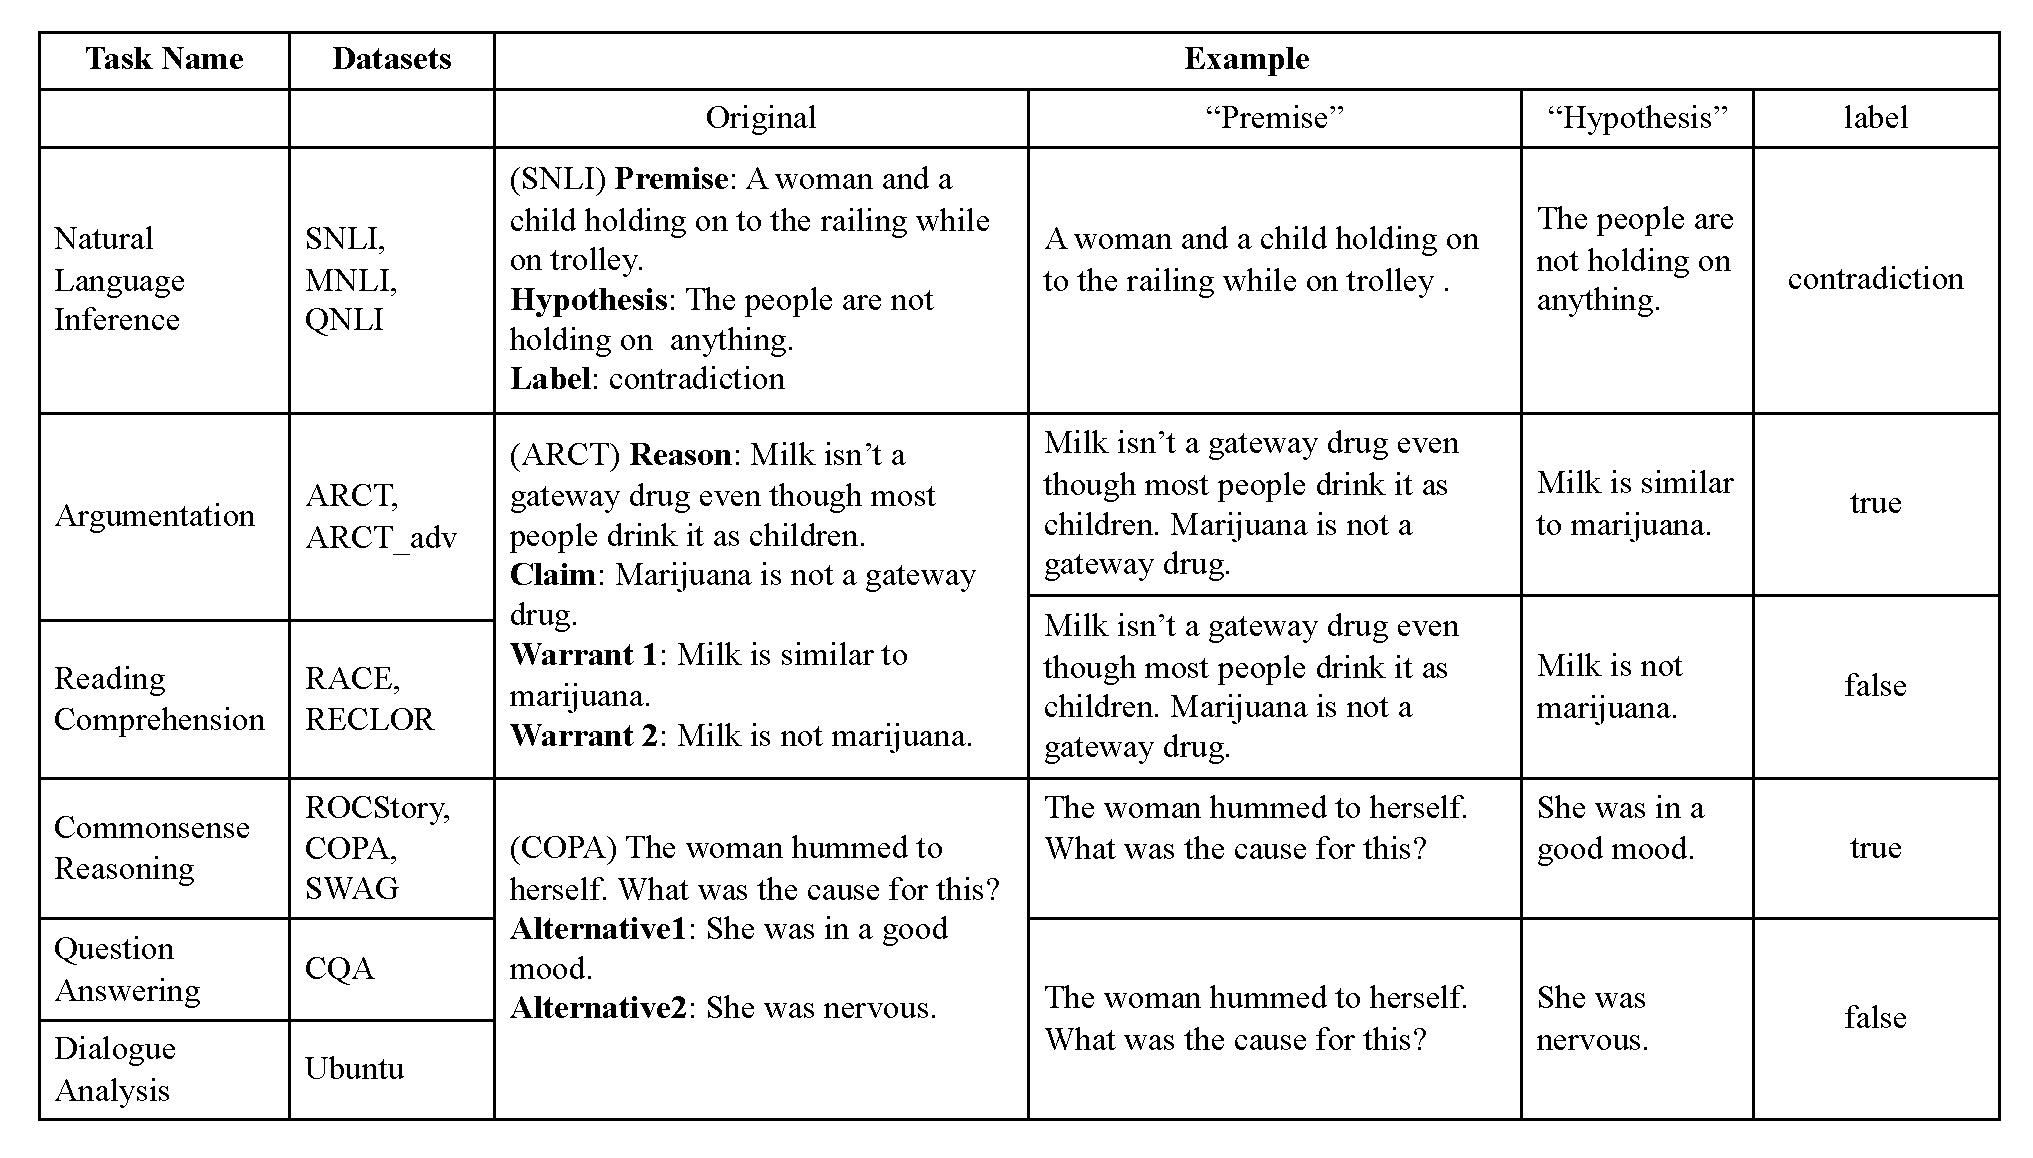
\includegraphics[width=2\columnwidth]{picture/datasets_exp.eps}
%\caption{Data examples and normalized version.}
%\label{tab:datasets_exp}
%\end{table*}
%

\subsection{Case Studies}
